\newpage
\section{Helmholtz problems}
\label{Sec:exteriorHelmholtz}
Recall that the Helmholtz problem is given by
\begin{alignat}{3}
	\nabla^2 p + k^2 p &= 0 	\quad &&\text{in}\quad \Omega,\label{Eq:HelmholtzEqn}\\
	\partial_n p &= g						&&\text{on}\quad \Gamma,\label{Eq:HelmholtzEqnNeumannCond}
\end{alignat}
where $\partial_n$ denotes the partial derivative in the normal direction, $\vec{n}$, on the surface $\Gamma$. For the exterior problem we must impose the Sommerfeld radiation condition~\cite{Sommerfeld1949pde} 
\begin{equation}\label{Eq:sommerfeldCond}
	\pderiv{p}{r}-\imag k p = o\left(r^{-1}\right)\quad \text{with}\quad r=|\vec{x}|\
\end{equation}
in order to restrict the field in the limit $r\to\infty$ uniformly in $\hat{\vec{x}}=\frac{\vec{x}}{r}$, such that no waves originate from infinity (to obtain uniqueness of the solution $p$).

A common approach for solving unbounded scattering problems with the FEM is to introduce an artificial boundary that encloses the scatterer. On the artificial boundary some sort of absorbing boundary condition (ABC) is prescribed. The problem is then reduced to a finite domain problem, and the bounded domain between the scatterer and the artificial boundary can be discretized with finite elements. Several methods exist for handling the exterior Helmholtz problem (on unbounded domain), including
\begin{itemize}
	\item the infinite element method (IEM)~\cite{Bettess1977ie,Bettess1977dar}
	\item local differential ABC operators~\cite{Shirron1995soe,Bayliss1982bcf,Hagstrom1998afo,Tezaur2001tdf}
	\item the perfectly matched layer (PML)~\cite{Berenger1994apm,Berenger1996pml}
	\item the boundary element method (BEM)~\cite{Sauter2011bem,Schanz2007bea,Marburg2008cao,Chandler_Wilde2012nab}
	\item Dirichlet to Neumann-operators (DtN-operators)~\cite{Givoli2013nmf}.
\end{itemize}
The initial formulation of the IEM assumed the artificial boundary to be a sphere. This restriction results in unnecessary large computational domains for elongated scatterers, and is somewhat relaxed in the ellipsoidal formulation after Burnett~\cite{Burnett1994atd,Burnett1998aea}, in which the infinite elements are attached on an ellipsoid as in~\Cref{Fig:model3_inWaterInf}. These formulations are the ones used in the second paper of this thesis. A further generalization of the artificial boundary was attempted in the work of Shirron and Dey~\cite{Shirron2002aie} where the artificial boundary may be any convex surface. For convex scatterer this enables the infinite elements to be attached directly onto the scatterer as in~\Cref{Fig:model3_in_waterInf2}. It is stated that this infinite element formulation preserves ``the accuracy (and convergence characteristics)'' of the IEM. A statement which can arguably be disputed as illustrated in the appendices as it very much so relies on the geometry of the artificial boundary. However, the reduced computational domain and simpler construction of the artificial boundary may be a sufficient compromise for the accuracy loss. 

\begin{figure}
	\centering
	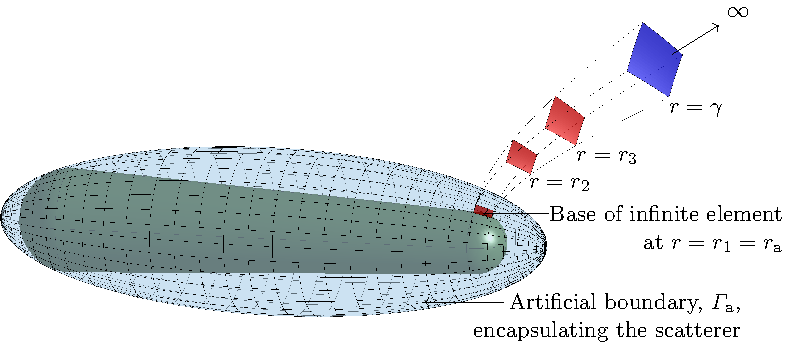
\includegraphics[width=\textwidth]{../../LaTeX/createFigures/TikzFigures/phd/model3_inWaterInf}
	\caption{An infinite element in a prolate spheroidal coordinate system.}
	\label{Fig:model3_inWaterInf}
\end{figure}
\begin{figure}
	\centering
	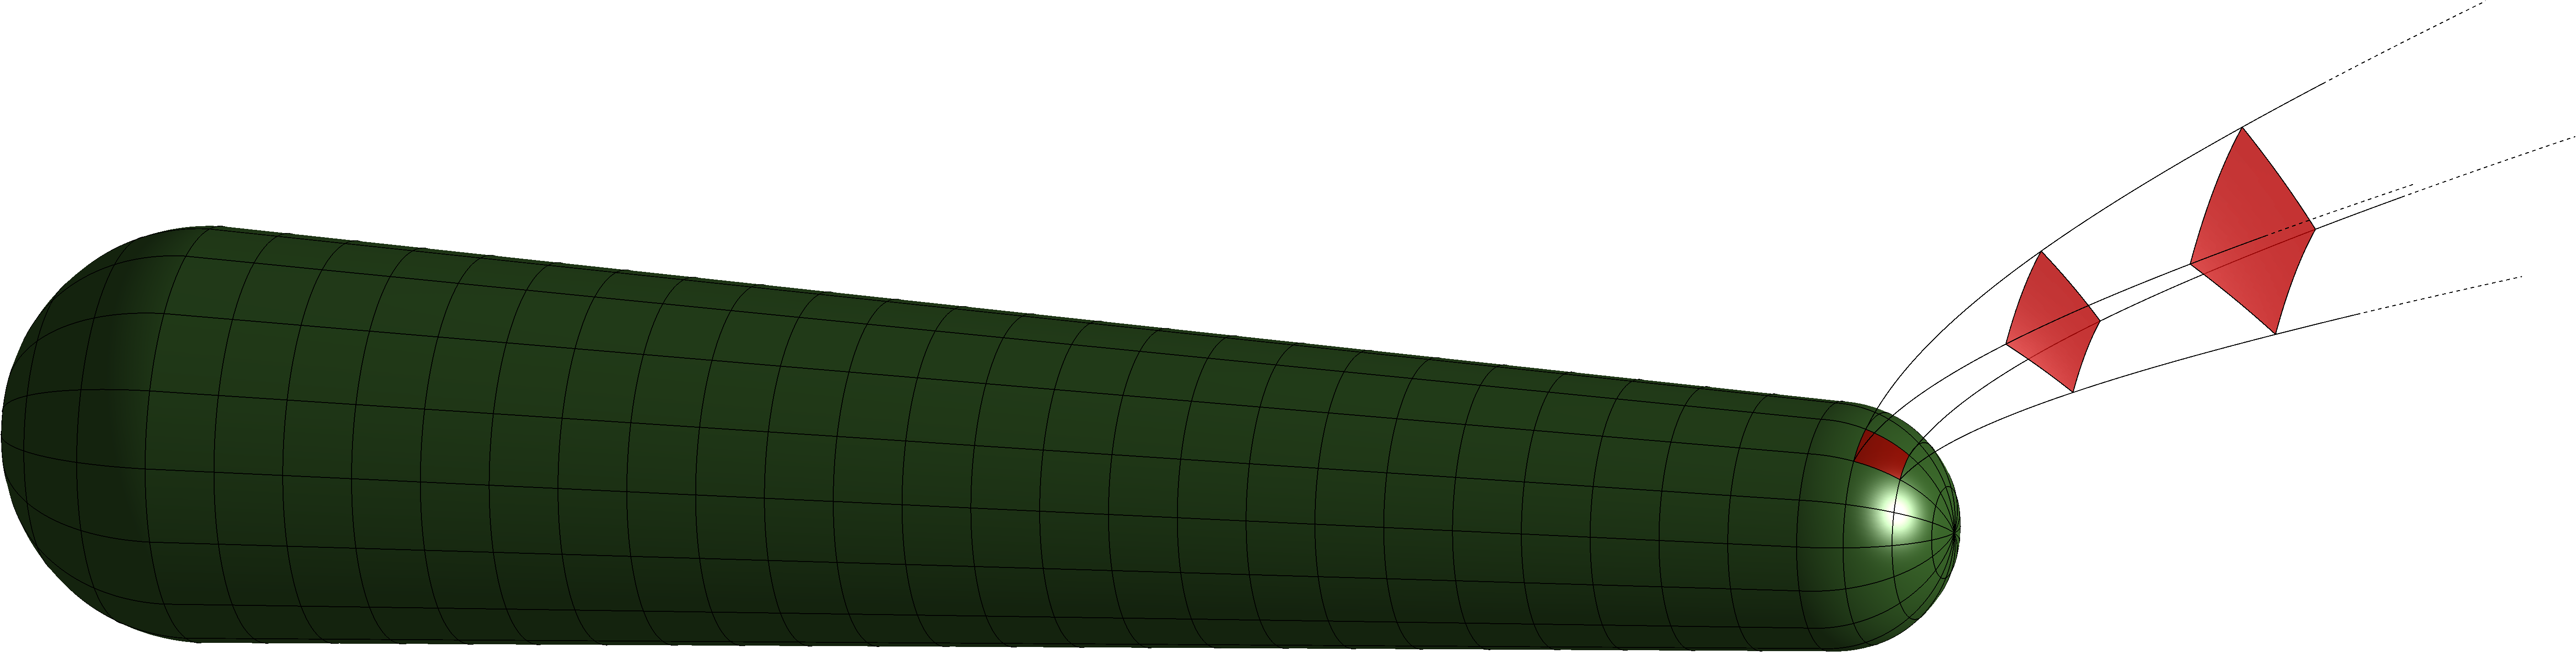
\includegraphics[width=\textwidth]{../../graphics/model3_in_waterInf2}
	\caption{An infinite element attached directly onto the scatterer (which is here the BeTSSi model 3).}
	\label{Fig:model3_in_waterInf2}
\end{figure}

The approach based on ABC operators has developed in much the same way as for the infinite elements with for example an artificial boundary of cigar shape presented in~\cite{Tezaur2001tdf}. Engineering precision ($\sim 1\%$) may be obtained by simple second order operators, but for higher accuracy the formulations becomes arguably more tedious to implement compared to the IEM as higher order derivatives are required. On the other hand, the conditioning of the system matrices for this approach is better than that of the infinite element method. Several attempts have been presented for the IEM to resolve the conditioning problem including~\cite{Dreyer2003ico,Safjan2001tic,Safjan2002tdi}. In~\cite{Safjan2002tdi} Safjan and Newman present basis functions with compact support (in the radial direction) also outside of the artificial boundary. Combining this approach with that of Shirron and Dey would be an approach to solve the conditioning problem while at the same time having lots of freedom to construct the artificial boundary.

The problems outlined above are not present for the BEM approach. Additionally BEM comes with several advantages including reduction of problem dimension (3D volume to 3D surface), no need to do surface-to-volume parametrization (thus, especially suited for IGA), and automatic incorporation of the Sommerfeld radiation condition. However, a host of new challenges arises. This includes fictitious eigenfrequencies, singular integrals and fully dense system matrices. All of which are presented in the third paper.

\subsection{Far field pattern}
The target strength (the quantity of interest) is defined in the far field and we are only solving for the near field. The Helmholtz integral equation gives us a convenient way to link these two fields.

If the field at the scatterer is known (i.e. after obtaining the solution numerically), one can compute the solution in the exterior domain, $\Omega^+$, using the following integral equation (cf.~\cite[Theorem 2.21]{Chandler_Wilde2012nab})
\begin{equation}\label{Eq:KirchhoffIntegral}
	p(\vec{x}) = \int_{\Gamma}\left[ p(\vec{y})\pderiv{\Phi_k(\vec{x},\vec{y})}{n(\vec{y})} - \Phi_k(\vec{x},\vec{y})\pderiv{p(\vec{y})}{n(\vec{y})}\right]\idiff \Gamma(\vec{y}),\quad\vec{x}\in\Omega^+
\end{equation}
where $\vec{y}$ is a point on the surface $\Gamma$, $\vec{n}$ lies on $\Gamma$ pointing ``into'' $\Omega^+$ at $\vec{y}$, and $\Phi_k$ is the free space Green's function for the Helmholtz equation in \Cref{Eq:HelmholtzEqn} given (in 3D) by
\begin{equation}\label{Eq:FreeSpaceGrensFunction}
	\Phi_k(\vec{x},\vec{y}) = \frac{\euler^{\imag kR}}{4\PI R},\quad\text{where}\quad R = |\vec{x} - \vec{y}|
\end{equation} 
with
\begin{equation*}
	\pderiv{\Phi_k(\vec{x},\vec{y})}{n(\vec{y})} = \frac{\Phi_k(\vec{x},\vec{y})}{R}(\imag kR-1)\pderiv{R}{n(\vec{y})}.
\end{equation*}
Using the limits (with $\vec{x}=\hat{\vec{x}}/r$ and $r=|\vec{x}|$)
\begin{equation}\label{Eq:Phi_k_limits}
\begin{aligned}
	&\lim_{r\to\infty} r\euler^{-\imag k r}\Phi_k(r\hat{\vec{x}},\vec{y}) = \frac{1}{4\PI}\euler^{-\imag k \hat{\vec{x}}\cdot\vec{y}}\\
	&\lim_{r\to\infty} r\euler^{-\imag k r}\pderiv{\Phi_k(r\hat{\vec{x}},\vec{y})}{n(\vec{y})} = -\frac{\imag k}{4\PI}\euler^{-\imag k \hat{\vec{x}}\cdot\vec{y}}\hat{\vec{x}}\cdot\vec{n}(\vec{y})
\end{aligned}
\end{equation}
the formula in \Cref{Eq:KirchhoffIntegral} simplifies in the far field to (cf.~\cite[p. 32]{Ihlenburg1998fea})
\begin{equation}\label{Eq:HelmholtzIntegralFarField}
	p_0(\hat{\vec{x}}) = -\frac{1}{4\PI}\int_{\Gamma}\left[ \imag k p(\vec{y})\hat{\vec{x}}\cdot\vec{n}(\vec{y}) + \pderiv{p(\vec{y})}{n(\vec{y})}\right]\euler^{-\imag k \hat{\vec{x}}\cdot\vec{y}}\idiff \Gamma(\vec{y}).
\end{equation}
from which the target strength in~\Cref{Eq:TS} may be computed.

%
%\subsection{Absorbing boundary conditions}
%\textcolor{red}{Give introduction to ABC and numerical example.}
%
%The ABC operator of first order is given by
%\begin{equation*}
%	\pderiv{u}{r} = \left(\imag k - \frac{1}{r_{\mathrm{a}}}\right) u 
%\end{equation*}
%and the second order operator by
%\begin{equation*}
%	\pderiv{u}{r} = \left(\imag k-\frac{1}{r_{\mathrm{a}}}\right) u + \frac{1}{2r_{\mathrm{a}}}\frac{1}{1-\imag kr_{\mathrm{a}}}\nabla_{\mathrm{S}}^2 u
%\end{equation*}
%the third is given by
%\begin{equation*}
%	\pderiv{u}{r} = \left(\imag k - \frac{1}{r_{\mathrm{a}}}\right) u + \frac{1}{2r_{\mathrm{a}}}\frac{1}{1-\imag kr_{\mathrm{a}}}\nabla_{\mathrm{S}}^2 u + \frac{1}{2}\frac{1}{1-\imag kr_{\mathrm{a}}}\frac{1}{2-\imag k r_{\mathrm{a}}}\left(2+\nabla_{\mathrm{S}}^2\right)\left[\left(\frac{1}{r_{\mathrm{a}}}-\imag k\right)u+\pderiv{u}{r}\right]
%\end{equation*}
%with
%\begin{equation*}
%	\nabla_{\mathrm{S}}^2 = \pderiv[2]{}{\vartheta} + \cot\vartheta\pderiv{}{\vartheta} + \frac{1}{\sin^2\vartheta}\pderiv[2]{}{\varphi}
%\end{equation*}
%
%Since (for the second order operator)
%\begin{equation*}
%	-\int_{\Gamma_{\mathrm{a}}} q\nabla p\cdot\vec{n}\idiff\Gamma = -\int_{\Gamma_{\mathrm{a}}} q\pderiv{p}{r}\idiff\Gamma = -\left(\imag k-\frac{1}{r_{\mathrm{a}}}\right)\int_{\Gamma_{\mathrm{a}}} qp\idiff\Gamma - \frac{1}{2r_{\mathrm{a}}}\frac{1}{1-\imag kr_{\mathrm{a}}}\int_{\Gamma_{\mathrm{a}}} q\nabla_{\mathrm{S}}^2p\idiff\Gamma
%\end{equation*}
%where
%\begin{equation*}
%	\int_{\Gamma_{\mathrm{a}}} q\nabla_{\mathrm{S}}^2p\idiff\Gamma = -\int_{\Gamma_{\mathrm{a}}} \nabla_{\mathrm{S}}q\cdot\nabla_{\mathrm{S}}p\idiff\Gamma
%\end{equation*}
%and
%\begin{equation*}
%	\nabla_{\mathrm{S}} = \frac{\vec{e}_{\upvartheta}}{r}\pderiv{}{\vartheta} + \frac{\vec{e}_{\upvarphi}}{r\sin\vartheta}\pderiv{}{\varphi}.
%\end{equation*}
%Since
%\begin{equation*}
%	\nabla_{\mathrm{S}}q\cdot\nabla_{\mathrm{S}}p = \frac{1}{r^2}\pderiv{q}{\vartheta}\pderiv{p}{\vartheta} + \frac{1}{r^2\sin^2\vartheta}\pderiv{q}{\varphi}\pderiv{p}{\varphi}
%\end{equation*}
%we get
%\begin{equation*}
%	-\int_{\Gamma_{\mathrm{a}}} q\nabla p\cdot\vec{n}\idiff\Gamma = -\left(\imag k-\frac{1}{r_{\mathrm{a}}}\right)\int_{\Gamma_{\mathrm{a}}} qp\idiff\Gamma + \frac{1}{2r_{\mathrm{a}}^3}\frac{1}{1-\imag kr_{\mathrm{a}}}\left[\int_{\Gamma_{\mathrm{a}}} \pderiv{q}{\vartheta}\pderiv{p}{\vartheta} + \frac{1}{\sin^2\vartheta}\pderiv{q}{\varphi}\pderiv{p}{\varphi}\idiff\Gamma\right]
%\end{equation*}
%
%The Bayliss-GunzBurger-Turkel-operators (BGT-operators)~\cite{Bayliss1982bcf}, are given by
%\begin{equation*}
%	B_N = \prod_{n=1}^N \left(\pderiv{}{r}-\imag k + \frac{2n-1}{r}\right) = \left(\pderiv{}{r}-\imag k + \frac{2N-1}{r}\right) B_{N-1}
%\end{equation*}
%such that we get the following boundary conditions
%\begin{equation*}
%	B_1 = \pderiv{u}{r}-\left(\imag k - \frac{1}{r}\right)u
%\end{equation*}
%\begin{equation*}
%	B_2 = \pderiv{u}{r}-\left(\imag k-\frac{1}{r_{\mathrm{a}}}\right) u - \frac{1}{2r_{\mathrm{a}}}\frac{1}{1-\imag kr_{\mathrm{a}}}\nabla_{\mathrm{S}}^2 u
%\end{equation*}
%where the second derivative is eliminated by the Helmholtz equation in spherical coordinates
%\begin{equation*}
%	\pderiv[2]{u}{r} = -\frac{2}{r}\pderiv{u}{r} - \nabla_{\mathrm{S}}^2 u - k^2 u.
%\end{equation*}
